\documentclass[10pt,a4paper]{article}
\usepackage[a4paper]{geometry}

\usepackage{polski}
\usepackage{indentfirst}
\usepackage{xltxtra}
\usepackage{relsize}
\usepackage{fancyvrb}
\usepackage[pdfborder={0 0 0}]{hyperref}
\usepackage{graphicx}

\defaultfontfeatures{Mapping=tex-text}
\setromanfont{Charis SIL}
\setmonofont[Scale=MatchLowercase]{Menlo}
\linespread{1.25}

\DefineVerbatimEnvironment%
  {SmallVerbatim}%
  {Verbatim}{fontsize=\relsize{-0.5},numbers=left,numbersep=-10pt,frame=lines,tabsize=4}

\newcommand{\ft}[1]{\texttt{#1}}

\begin{document}

%%fakesection{Tytuł}
\title{ 
  Interpolacja funkcjami sklejanymi\\
  {\normalsize Specyfikacja implementacyjna projektu nr 2}\\\vspace{-12pt}
  {\normalsize z przedmiotu \emph{Języki i metody programowania 2}}
}
\author{
  Tomasz Cudziło\\
  {\small EE PW, 211552}
}
\date{\today}
\maketitle

\section*{Zadanie}
\label{sec:zadanie}

Napisać program, z~graficznym interfejsem użytkownika, wyznaczający
współczynniki funkcji sklejanych trzeciego stopnia aproksymujących zadany ciąg
danych pomiarowych.

\vspace{20pt}

\section{Logika klas}

Cały projekt jest luźno oparty na wzorcu \ft{MVC}. Punktem wejścia jest klasa
\ft{SplinesApp}, która posiada obiekt klasy \ft{SplinesController}. Ta
instancja kontrolera, posiada obiekty punktów, wielomianów i~wykres, oraz
zarządza nimi zgodnie z~poleceniami użytkownika płynącymi z~instancji
\ft{SplinesView}.

Schemat z~rys.~\ref{fig:aplikacja} na stronie \pageref{fig:aplikacja}
przedstawia zarys podziału problemu na klasy.

\begin{figure}[hp]
  \centering
  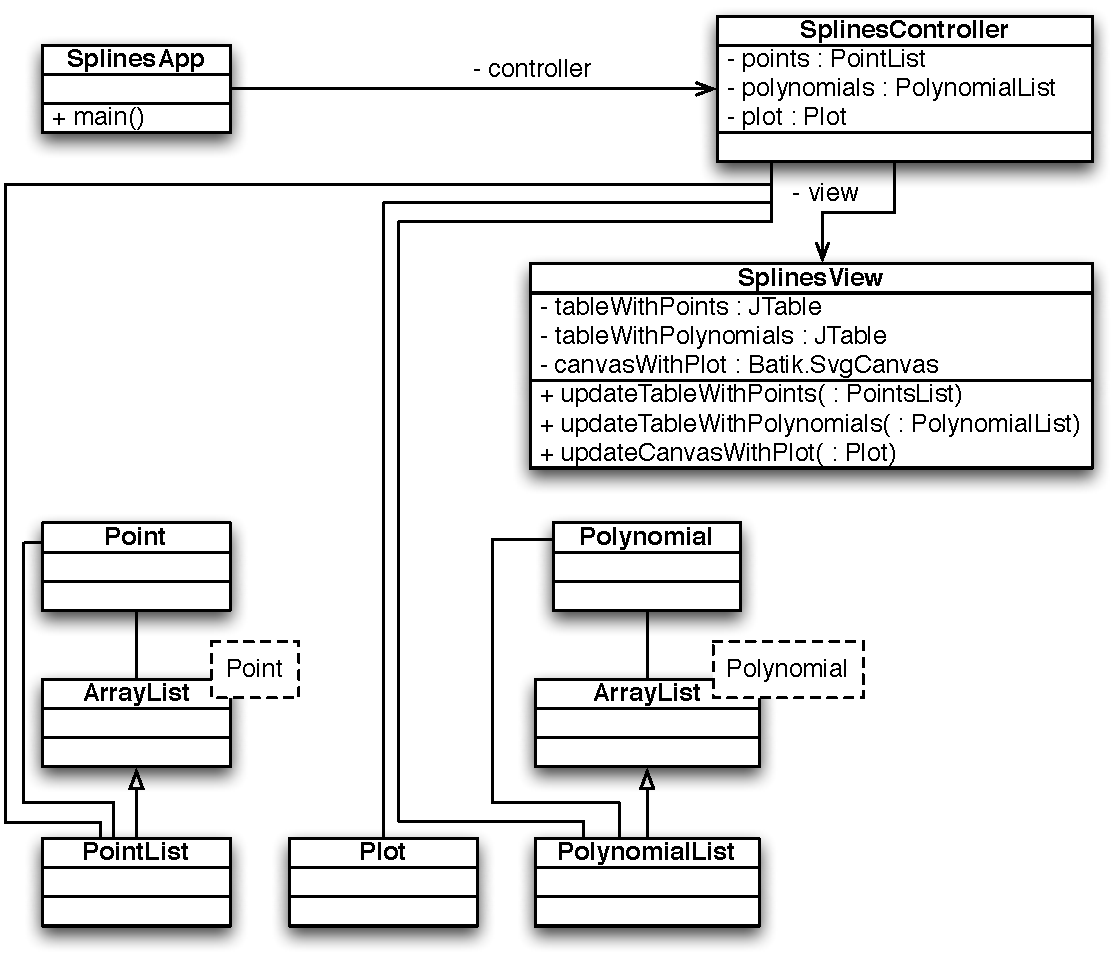
\includegraphics[width=\textwidth]{figury/aplikacja}
  \caption{Schemat całej aplikacji.}
  \label{fig:aplikacja}
\end{figure}

\subsection{Modele}

\subsection{Kontroler}

\subsection{Widok}

\section{Pliki}

\end{document}
